%************************************************
\chapter{Introduction}\label{ch:intro}
%************************************************

\tikz[remember picture,overlay] \node[opacity=0.3,inner sep=0pt] at (current page.center){\includegraphics[width=\paperwidth,height=\paperheight]{./Figures/cover/sesshu_11.jpg}};
\clearpage

\section{Community Ecology}

Humans have always marveled at the diversity of life forms on Earth. This fascination is reflected in the multitude of ways in which nature is represented and studied in the different branches of human knowledge. Some enjoy looking at the finest detail of the life histories of species and populations. To some of us, life forms are inherently self-organized into larger-scale structures that display their own rules and meaning; thus we look at a forest and see, indeed, a tight entanglement of individuals that cannot possibly thrive without the surrounding web of other species. Individual details, while extremely important, are embebbed into entities that posses their own ecological, aesthetical and etical relevance: ecological communities. While the Clementsian extreme view of communities as full-fledged, delimited entities capable of evolution and reproduction has long been abandoned, it is obvious that associations of individuals do generate predictable sets of processes and patterns, and the main concern of community ecology is with the discovery and understanding of these general processes and patterns. Community ecology is the discipline most directly concerned with the temporal and spatial scales at which individuals interact with each other. Processes intrinsic to this scale are generated by individual-level behaviours, that shape interaction patterns. Whatever the mechanisms by which such community-level patterns are driven, they feedback and influence individual life histories and, in turn, also biogeographic and macroecologic processes, such that the study of community ecology has an important relevance on its own and also plays a key role in understanding the emergence of global patterns from lower-scale processes.

Intuitively, an ecological community can be defined simply as a set of individuals that interact with each other. This broad picture needs to be refined when addressing the systematic study of these entities. For example, how do we define the \textit{set} of species that constitutes a community? What are the \textit{spatial} and \textit{temporal} limits of a given community? In the first chapter of this thesis, for example, we will encounter a community located on a small islet, in which a top predator is a bird of prey that can easily travel dozens of kilometers in a single journey and is thus not constrained by the territory of the islet, whereas other species are sessile or limited to ranges of a few hundreds of meters. Why would I include this top predator as part of the island community, when it clearly has a broader range than the rest of the species? And, looking at this question from another point of view, why would I \textit{not} consider as part of this community other species outside the islet that are also preyed upon by this predator?

The answer, as almost always in ecology, is that no fixed rules are applicable to all cases. Communities, despite their inherent structure and identity, are not organisms with closed physical boundaries to the outside world, and therefore, their spatiotemporal borders are extremely variable and are usually chosen ad-hoc by the investigators studying them. A great deal of studies in community ecology deal with so-called \textit{horizontal} communities. These are simply communities composed of organisms of similar characteristics, usually in terms of taxonomical relatedness. Thus, it is very easy to find studies about the \textit{grassland} communities of a steppe, or about the \textit{arthropod} communities present on the canopy of tropical trees. Such focus on certain groups of related species is necessary in order to understand in detail certain ecological processes and patterns, such as niche differentiation and coexistence among similar species. It is also very convenient in terms of experimental design, as it allows investigators to concentrate efforts on a small part of the enormous diversity present in every habitat. Studies on horizontal communities are at the core of classic community ecology, and we have learnt much about how species coexist with each other when resources are limited, about how species are positioned along environmental gradients, and about many other ecologically relevant questions.

Notwithstanding the importance and validity of the abstraction of horizontal communities, it is clear that they are somehow incomplete communities, if we recall the broad definition of community sketched above. No one can doubt that, in natural settings, the group of e.g. grassland species is interacting in many ways with other guilds: they are consumed by arthropod or mammal herbivores differentially, they may be pollinated by other sets of species, they may be affected by stamping of big animals or be fertilized by their dung. All in all, communities are more than disjointed taxonomic guilds, and their dynamics are influenced by the whole set of interactions occurring among their constituent species. The role of interspecific interactions is, then, key for understanding and predicting important ecological processes at this scale. It is this vision that has given rise to another long-standing branch of community ecology that has at its core the study of the interactions between different guilds or species within a community: the study of ecological networks. This thesis deals with complex communities represented as networks of interacting species, so I will give a brief overview of network theory in general and applied to ecological communities, and later introduce the specific questions addressed in this thesis.

\section{Communities as ecological networks}
\subsection{Network theory}

Network theory is a branch of applied mathematics that studies the relations between discrete entities, and the emergent properties and structures from these relations. Network theory is generally considered a subset of graph theory, with the main difference between them being that graph theory is more focused on the abstract behaviour of graph classes, whereas network theory is mainly applied to empirical systems and, thus, puts a strong emphasis on the dynamics of the system and its relationship with its structure. The first study that laid the foundation of graph theory is the famous problem of the Seven Bridges of Königsberg formulated and solved negatively by Euler in 1736, and graph theory developed steadily from that initial study. The application of graph theory to complex networks and their dynamics has grown enormously in, specially, the last decades of the 20th century, up to the point that nowadays the study of complex networks is an integral part of a multitude of scientific fields, from social and economic sciences, applied physics or robotics, to virtually every branch of biological sciences. Here I will provide very brief definitions of concepts that will be useful for understanding ecological networks in general and the investigations of this thesis in particular. It is not my intention to provide a comprehensive introduction to network theory (the reader is referred to \cite{Newman2010} and \cite{Barabasi2016} for overviews on that general topic), but rather to review the basics from which ecological networks can be understood and analyzed.

%\begin{scriptsize}
%\marginpar{
%{\color{Gray}
%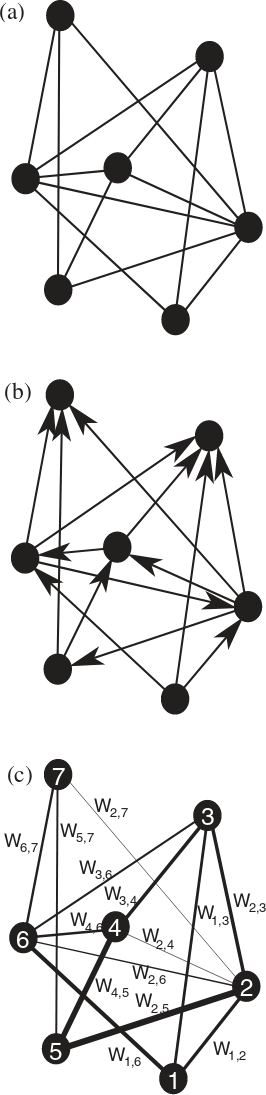
\includegraphics[width=\marginparwidth]{./Figures/intro/network_theory/graph_properties_Boccaletti2006.png}
%\captionof{figure}[Three types of graphs]{An undirected (a), a directed (b), and a weighted undirected (c) graph. From \cite{Boccaletti2006}}
%}
%}
%\end{scriptsize}

Starting with the building blocks of networks, we may define a \textbf{graph} as a pair of sets $G = (V,E)$, where $V = \{v_1,v_2,...,v_n\}$ is the set of \textbf{nodes} of the graph, and $E$ is the set of \textbf{edges}, or links, of the graph connecting pairs of nodes. The set $E$ can be any subset of all ordered pairs of $V$, such that $E \in V \otimes V$. Graphs can be either \textbf{directed} or \textbf{undirected} depeding on whether their constituent links are directional, i.e. whether $[v_i,v_j] \in E$ implies $[v_j,v_i] \in E$ (Fig. 1.1). Further, simple graphs are antirreflexive, meaning that a node cannot be linked to itself, i.e. $[v_i,v_j] \in E$ implies $i \neq j$.

Such a simple configuration can be easily extended by considering weighted or quantitative links. By incorporating weights, a \textbf{weighted graph} is a quadruple $G = (V,E,W,f)$, where $V$ and $E$ are the sets of nodes and edges defined above, $W = \{w_1,w_2,...,w_n\}$ is a set of weights such that $w_i \in \mathbb{R}$, and $f: E \rightarrow W$ is a mapping assigning weights to edges.

Intuitively, we say that two nodes $v_i$ and $v_j$ are \textbf{adjacent} to each other, or connected, if they are joined by an edge $e = \{v_i,v_j\}$. Similarly, two edges are adjacent if they are incident to at least one node.

The most basic structural property of a node is its \textbf{degree}. It is defined simply as the number of links incident to it. In directed graphs, one may distinguish in-degree, the number of links incident to a node, from out-degree, the number of links incident from it.

\begin{figure}[ht]
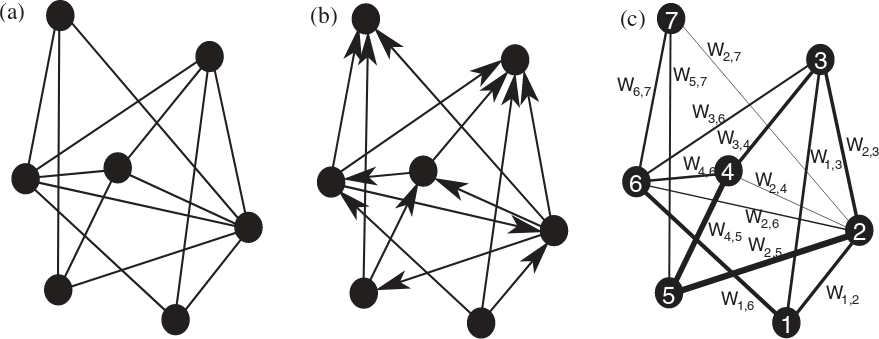
\includegraphics[width=\textwidth]{./Figures/intro/network_theory/graph_properties_Boccaletti2006_horizontal.png}
\caption[Three types of graphs]{An undirected (a), a directed (b), and a weighted undirected (c) graph. From \cite{Boccaletti2006}}
\label{fig:network_types}
\end{figure}

The \textbf{shortest path} connecting two nodes $v_i$ and $v_j$ is defined as the path with the shortest number of edges that connects them. This quantity, $L_{min}$, is also called the \textbf{distance} between two nodes. For weighted graphs, this definition may be refined to consider edge weight, such that the shortest path is the one that minimizes the summed weight of the edges connecting the two nodes.

A graph, in the context of network theory, is termed a \textbf{network}, and we will use this term hereafter. A network is said to be \textbf{complex} when it possesses topological features that are neither random nor completely regular. These features refer to properties of the network as a whole, and three of the most widely studied features of network are their degree distribution, their average path length and their clustering coefficient.

The \textbf{degree distribution} of a network is the probability distribution of the degrees of the network nodes. It is an important property of complex networks, as the degree distributions of random networks differs systematically from that of empirical networks of different types \citep{Barabasi1999}. While randomly assembled networks display Poisson degree distributions, many real networks are best represented as having power-law degree distributions. This means that in real networks, most nodes are typically connected to only a few other nodes (i.e. have a low degree), whereas a small number of nodes are highly connected. Networks with power-law degree distributions are alternatively called \textbf{scale-free networks} (Fig. \ref{fig:scale_free}).

\begin{figure}[ht]
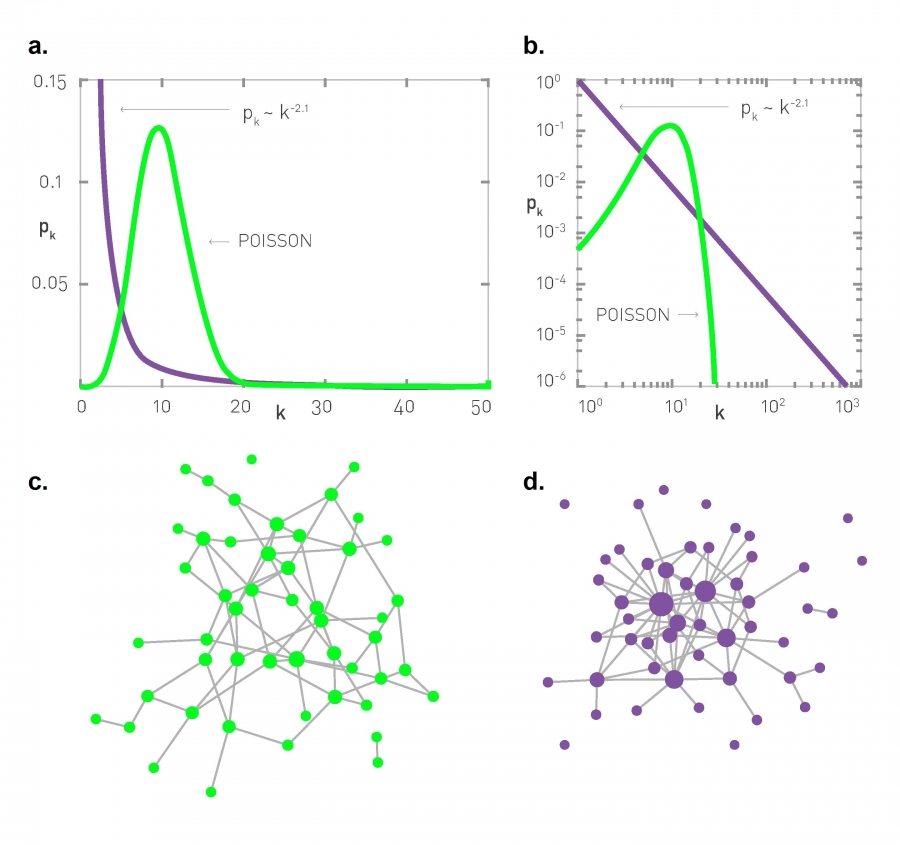
\includegraphics[width=\textwidth]{./Figures/intro/network_theory/degree_distrib_Barabasi2016.jpg}
\caption[Random and scale-free degree distributions]{\color{Gray} Degree distributions from random (green) and scale-free networks (purple) in natural (a) and logarithmic (b) axes. The hubs present in scale-free networks are evident in the network depiction (d). From \cite{Barabasi2016}}
\label{fig:scale_free}
\end{figure}

The \textbf{average path length} of a network is the average of the shortest paths between each pair of network nodes. It is given by

\begin{equation}
L = \frac{1}{S(S-1)} \sum_{i,j=1,S;i \neq j} L_{min}(i,j)
\end{equation}

and gives a measure of connectedness between any pair of nodes. Both random and scale-free networks display characteristically short average path lengths \citep{Montoya2002}.

Another important topological property is the \textbf{clustering coefficient}. It measures the degree to which the neighbours of a given node are linked together. Given a node $i$ with degree $d_i$, its local clustering coefficient is defined as

\begin{equation}
C_v(i) = \frac{2E_i}{k_i(k_i - 1)}
\end{equation}

where $E_i$ is the number of links between the $k_i$ neighbors of node $i$. The clustering coefficient of the network is the average over all $S$ nodes:

\begin{equation}
C_v = \frac{1}{S} \sum_{i=1}^{S} c_v(i)
\end{equation}

When considering network topology, networks without any differentiation between nodes, where each node can in principle interact with any other node, are called \textbf{unipartite}. Another common type of ecological networks is that which represents two disjoint groups that interact with each other but not with members of the same group (for example, a network with a group of plant species and a separate group of pollinators, Fig. \ref{fig:bipartite_nested}). Such networks are called \textbf{bipartite}.

\begin{figure}[ht]
\centering
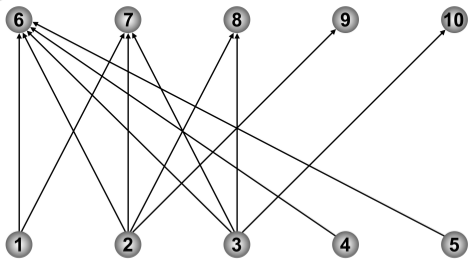
\includegraphics[width=0.5\textwidth]{./Figures/intro/network_theory/bipartite_nested_network_Ings2009.png}
\caption[Nested bipartite network]{\color{Gray} A bipartite network, in which nodes 1-5 and nodes 6-10 form sets that do not have within-group links. The network is also nested: the diet of consumer 8 is a subset of that of consumer 7, which in turn is a subset of that of consumer 6. From \cite{Ings2009}}
\label{fig:bipartite_nested}
\end{figure}

Several other network properties are widely used in the context of ecological networks. Here I will mention three of them. First, the \textbf{connectance} of a network is the proportion of realized links with respect to the potential number of links in the network. It is defined in different ways depending on the assumptions about the feasible links of the network. Four variations are possible regarding the directedness of the network and the feasibility of self-loops. The most general case is a directed network where self-loops are allowed. In that case, the set of potential links is simply $L_p = S^2$ for a network of $S$ nodes. If self-loops are not allowed, the set of potential links is $L_p = S^2 - S$, whereas if the network is undirected, the number of potential links halves, i.e. $L_p = S^2/2$. Therefore, an undirected network with no self-loops has $L_p = (S^2 - S)/2$ potential links. The general definition of connectance is

\begin{equation}
C = \frac{L}{L_p}
\end{equation}

where $L$ is the number of realized links.

The above definitions of the set of potential links imply that, aside from the consideration of self-loops, all links between any pair of species are potentially feasible.

Another topological property widely studied, \textbf{modularity} is the tendency of the network to display modules highly connected within but largely disconnected from each other. The detection of modules, or clusters, in networks is an active area of research, and a closed definition of modularity depends on the expected number of modules and their link distribution. As an example, \cite{Fortuna2010} defined modularity as

\begin{equation}
M = \sum_{s = 1}^{N_M} \left[\frac{l_s}{L} - \left(\frac{d_s}{2L}\right)^2\right]
\end{equation}

Lastly, \textbf{nestedness} is a property of bipartite networks by which nodes with low degree are connected to a subset of the nodes linked by nodes with high degree (Fig. \ref{fig:bipartite_nested}).

Aside from these general definitions, it is important to mention the matrix representation of networks. Intuitively, by defining a matrix $A$ of dimensions $S * S$, its entries $a_{i,j}$ may represent the existence (or weight) of a link between nodes $i$ and $j$. Such matrix is called the \textbf{adjacency matrix}. If the network is undirected, its adjacency matrix is symmetric, i.e. $a_{i,j} = a_{j,i}$

\[
A_{undirected} = \begin{pmatrix}
0& 1& 0 \\
1& 0& 1 \\
0& 1& 0
\end{pmatrix}
\]

where $a_{i,j} = 1$ if a link exists between nodes $i$ and $j$, and $a_{i,j} = 0$ otherwise. If the network is directed, the possibility exists that $a_{i,j} \neq a_{j,i}$, so that an example matrix can be

\[
A_{directed} = \begin{pmatrix}
0& 1& 0 \\
0& 0& 0 \\
1& 1& 0
\end{pmatrix}
\]

The convention for directed networks is that adjacency matrices represent the interaction originating in column $j$ and affecting row $i$, so that in the previous example, there is a link from node 2 to node 1, but not the other way around. %The matrix formulation of networks has particular importance in evaluating the stability properties of the associated system, and thus has been extensively used in studies of ecological dynamics. In the next section, I briefly review early developments on ecological networks and further develop some of the properties defined above.

\subsection{Ecological networks: brief history, recent developments and open questions}

The general definitions outlined above can be applied to ecological systems seamlessly by defining individuals, species or guilds as nodes, and the biotic interactions among them as the edges or links connecting them. Indeed, natural historians and early ecologists had recognized the network nature of ecological communities long before the recent developments on complex networks. The brief historical review that follows draws primarily from the works by \cite{Bersier2007} and \cite{Ings2018}, and the reader is referred to these studies for consulting primary references.

The first documented observations about the interactions of species can be traced back to Ancient Greece, where mutualistic relationships were observed by Herodotus, Theophrastus and Aristotle. In turn, the arab scholar Al-Jahiz is believed to have introduced the concept of food chain in his \textit{Book of the Animals}, in the 9th-century. In the early Enlightenment the documented study of the natural world began to gain back attention, although admittedly on a secondary position with respect to mathematics, physics, chemistry or astronomy, disciplines that constituted the main focus of the Scientific Revolution. Observations about empirical food chains are documented by van Leeuwenhoek and Linnaeus, but it would be Alexander von Humboldt in the 19th-century, throughout all his works, the first and most influential proponent of a view of nature that emphasized the complex web of relationships between species, looking at nature as a ``living whole''. The first representation of a full network of trophic interactions dates from 1880, and was made by the italian scientist Lorenzo Camerano.

After these and other seminal contributions, the 20th-century saw the confirmation of network-oriented approaches to ecological issues. The ecologist Charles Elton developed many important concepts, such as the ``pyramid of numbers'' by which abundances decreased along the food chain, and established the terms \textit{food chain} and \textit{food cycle}. After his seminal works, the network representation of trophic relationships became a common framework for studying ecological communities. By this point, trophic relationships were already the most studied interactions in ecological communities. Trophic interactions are ubiquitous in nature, they are usually the easiest to document and, unlike other interactions, can be used to outline the fluxes of biomass and energy in a given community. It is, therefore, not surprising that they took, and still maintain, such a predominant role in studies of ecological networks. The figure of Raymond Lindeman also stands out in the first half of the 20th century, with his work ``The trophic dynamic aspect of ecology'', in which he studied for the first time the quantitative fluxes and feedbacks between the biotic and abiotic components of an entire ecosystem, the Cedar Bog Lake in Minnesota \citep{Lindeman1942}. As \cite{Ings2018} note, limnology had a prominent position on these early developments, and many temperate lakes were the first ecosystems to be thoroughly sampled and studied.

In parallel to these insights from natural systems, the mathematical foundations for studying the dynamics of ecological interactions were being developed. The mathematician Alfred J. Lotka proposed in 1920 a set of equations for the population dynamics of a pair of predator and prey species, that explained the apparent oscillations observed in plant-herbivore systems \citep{Lotka1920}. In an independent contribution another mathematician, Vito Volterra, derived similar equations following observations of fish catches in the Adriatic Sea \citep{Volterra1928}. The general form of these equations is

\begin{equation}
\begin{array}{c}
\frac{dx}{dt} = \alpha x - \beta xy \\
\frac{dy}{dt} = \delta xy - \gamma y
\end{array}\label{eq:LV}
\end{equation}

where $x$ is the number of prey, $y$ is the number of predators, $\alpha$ is the growth rate of the prey, $\beta$ the predation rate coefficient, $\delta$ the predator's growth rate, and $\gamma$ its mortality rate. In this model, both species modulate their abundances in response to the other (Fig. \ref{fig:LV_example}), and the non-trivial solution to the system, formulated as with eq. \ref{eq:LV} is stable and periodic. The Lotka-Volterra set of equations implies a series of assumptions about the underlying biological system. First, they are an example of a mean-field system, thus assuming an homogeneous habitat in which individuals are interacting without constraints or variations. Prey populations in the absence of the predator display exponential growth (i.e., if $ y = 0$, the variation in prey density is given by $\alpha x$), and the predator depends entirely on the prey population. Furthermore, predators do not satiate, in that they respond instantaneously to increases in prey population. Importantly, all $\alpha , \beta , \delta , \gamma$ coefficients are constant, thus assuming no other sources of variation.

\begin{figure}[ht]
\centering
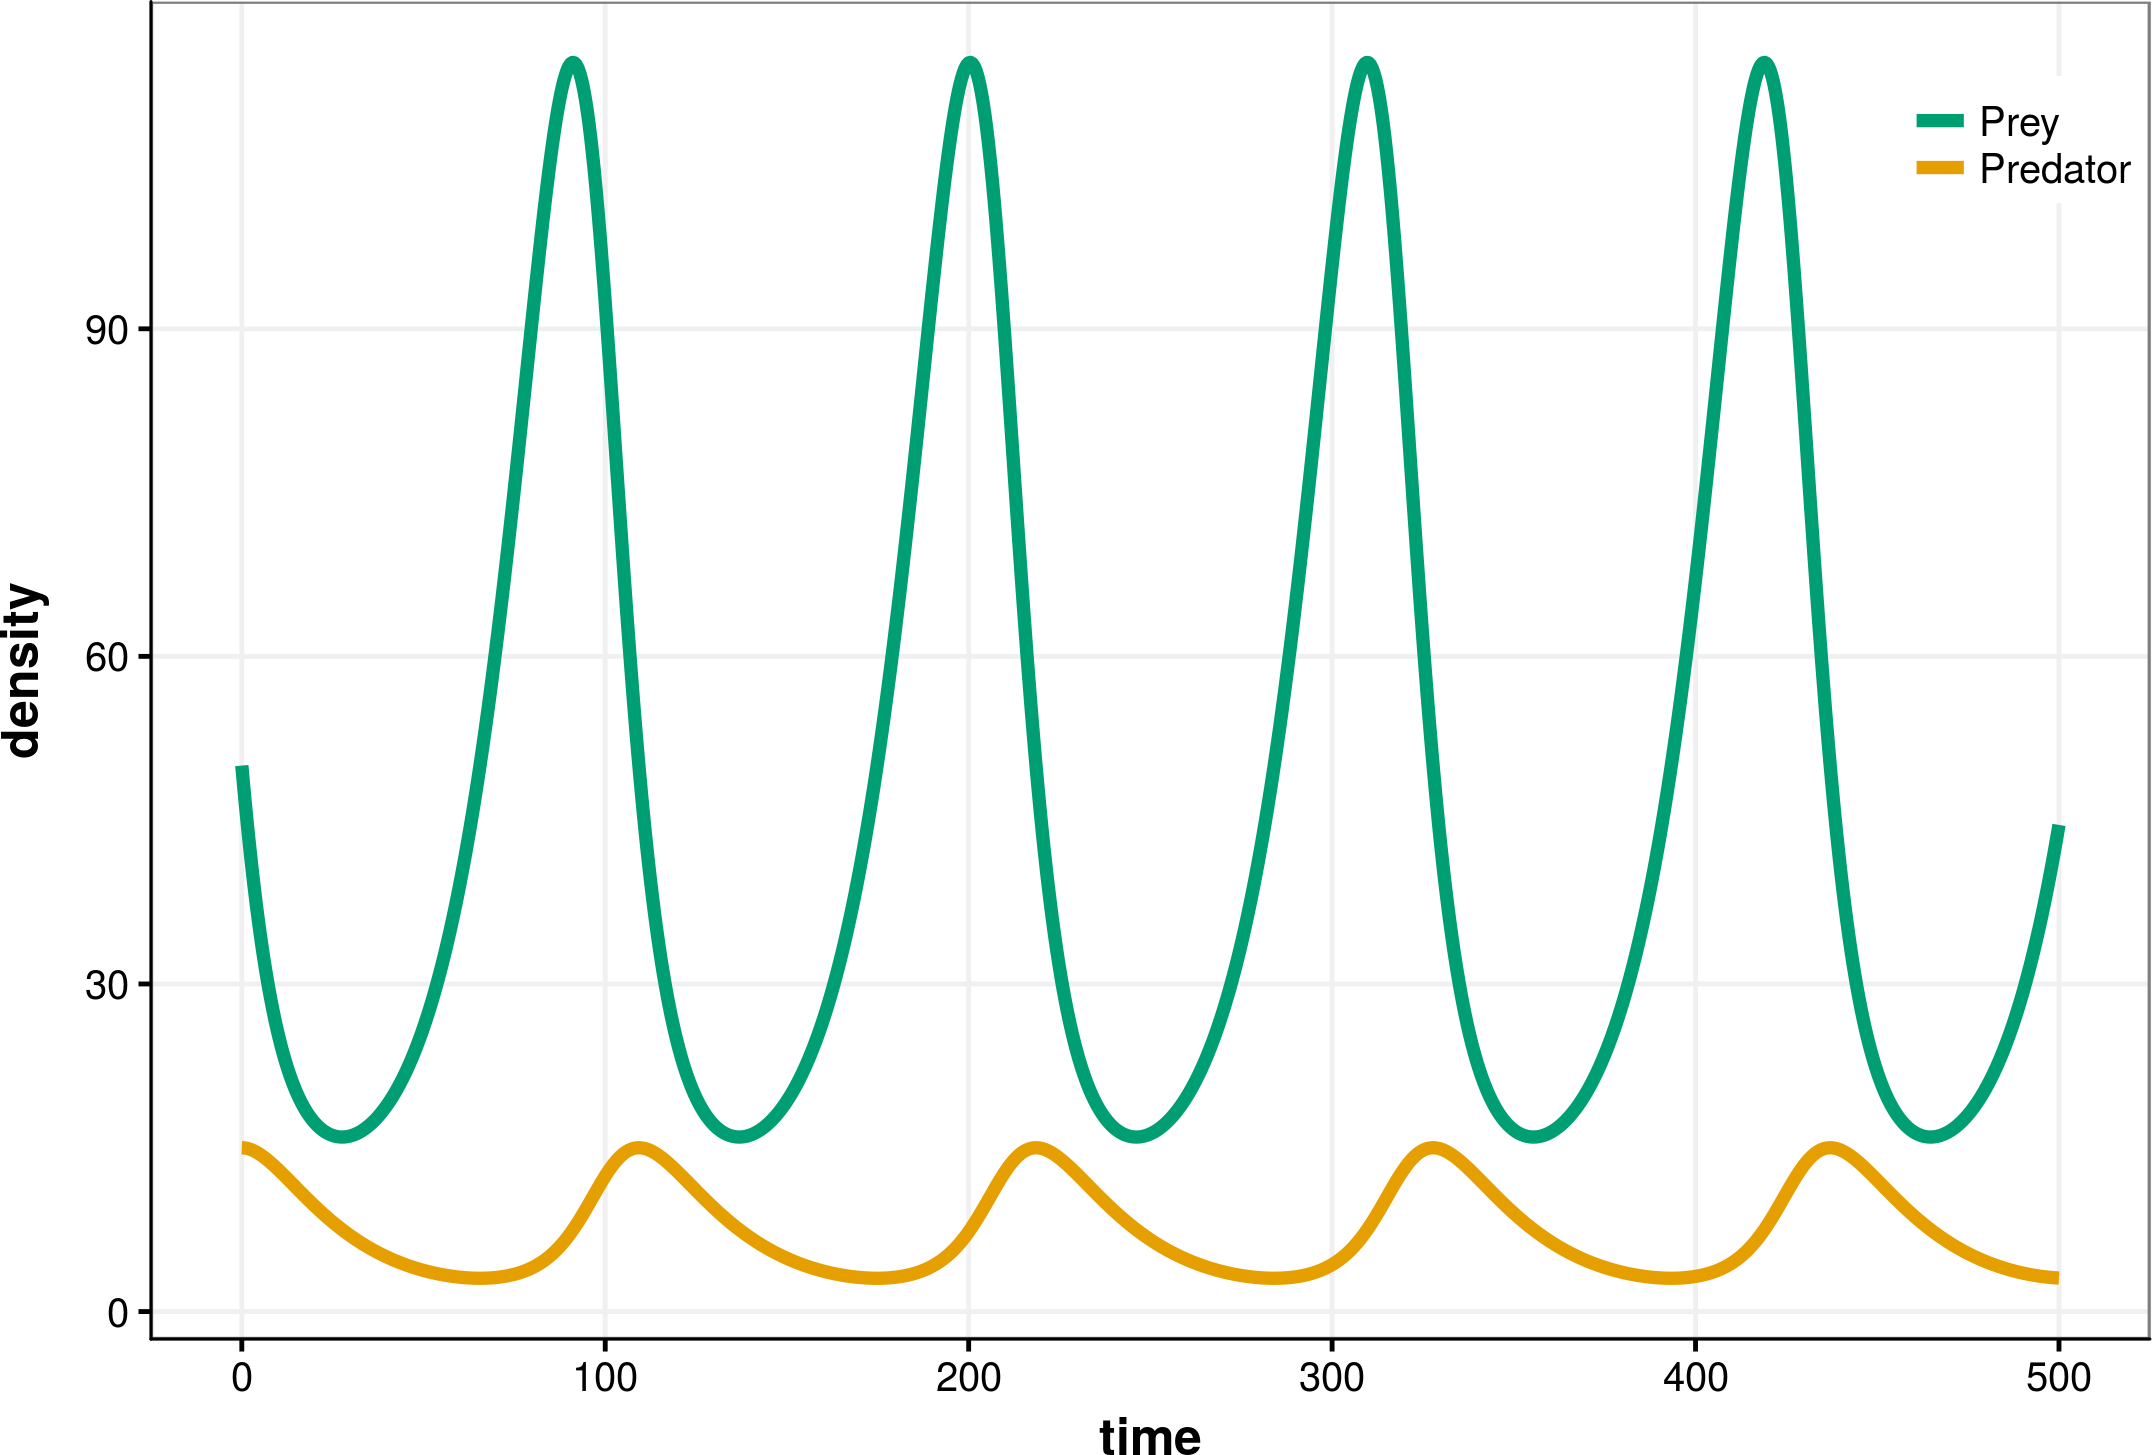
\includegraphics[width=.75\textwidth]{./Figures/intro/ecological_networks/LV_example.png}
\caption[2-species Lotka-Volterra system]{\color{Gray} Lotka-Volterra equations generate stable population dynamics in which densities of the prey and the predator species are both dependent on each other.}
\label{fig:LV_example}
\end{figure}

In the context of dynamical systems, the stability of the system can be approached by analysing how the system responds to very small perturbations off a steady state. This is done by calculating the \textit{eigenvalues} of the system, values that encapsulate the response of the system to such a small perturbation around the equilibrium. The mathematics behind the calculation and interpretation of eigenvalues have been thoroughly developed, and the interested reader may find innumerable derivations of it. In the context of ecological networks, the book \textit{Food Webs} by Kevin \cite{McCann2011} gives a well-balanced introduction to the study of dynamical systems. The important message is that the eigenvalues of a dynamical system (in particular, the maximum eigenvalue) are informative about the stability of the system. Positive eigenvalues will imply that the system is locally unstable, whereas negative eigenvalues mean that the system is locally stable around that particular equilibrium.

Despite the initial insights from 2-species model systems, many ecologists were, as we have seen, much more interested on the notion of stability of whole communities or ecosystems. The first conceptual treatments of community stability can be traced back to Eugene Odum, who suggested that in a community, the number of alternative paths a quantum of energy has for going from primary producers to top predators is a measure of the stability of the community. This notion that the more links an ecological network had, the more stable it was (or, in other words, that ``complexity begets stability''), was the prevalent opinion up until the early 70s. Robert MacArthur, in another highly influential study, analyzed the stability of complete food webs in a semi-quantitative way. He arrived to the hypothesis that community stability increases by either increasing the number of species in a community, or the connectance of the associated food web \citep{MacArthur1955}.

The complexity-stability dichotomy of ecological communities entered a new dimension after the seminal work of Robert May \citep{May1972}, who used for the first time mathematical models of idealized communities to assess the local stability of systems with an indeterminate number of species modelled with Lotka-Volterra dynamics. He found that, in randomly assembled networks with normally distributed interaction strengths, the dynamical systems remain locally stable if

\begin{equation}
\alpha \sqrt{SC} < 1\label{eq:May}
\end{equation}

where $\alpha$ is the average interaction strength, $S$ is the number of species, and $C$ is the connectance of the network in the form $L/S^2$. The interpretation is that an increase in either mean interaction strength of the system, species richness, or number of links, would rapidly tend to destabilize the system. Crucially, May was of course aware of the limitations of his approach: the assembled networks possessed no structure whatsoever, pairwise interaction strength was assumed to be a constant, stochastic parameter, and the definition of stability involved infinitesimally small perturbations from an equilibrium state, as given by the eigenvalues of the system. Nevertheless, regardless such obvious limitations, May's work was the first quantitative derivation about the expected stability of arbitrarily large ecological communities, and not only so, but it also was a frontal attack on the common wisdom championed by MacArthur (who passed away way too early, in 1972) and many others by that time. The debates and number of studies triggered by May's results are countless, both in the camps of the theoreticians and the empiricists. From that moment onwards, the study of ecological networks started to gain even more attention and took many different parallel paths. An important line of research, that did not start with May's results but definitely gained attention after them, follows the estimation of interaction strengths both in theoretical studies of functional responses \citep{Holling1965} and empirical estimations \citep{Bender1984}.

Robert Paine showed in 1966 that the effects of removing a top predator could propagate throughout the whole ecological network, eventually altering the richness of the community \citep{Paine1966}. This striking result led to the denomination of \textit{keystone species} to those species with a disproportionate influence in the overall structure and dynamics of the community. He continued to be interested in measuring the impacts of one species over another and on the overall community, a theme that came together with the theoretical importance of interaction strength proposed by May. Theoretical metrics of interaction strength represent changes in different per capita or population-level parameters \citep{Laska1998} but such metrics are, importantly, not generally equivalent to what is measured in experimental studies (e.g. \citealt{Bender1984}). Paine observed that descriptions of food webs that failed to account for estimates of interaction strengths were not enough in order to link the structure of food webs with their dynamical behaviour \citep{Paine1992}.

However, obtaining empirical estimates of all interaction strengths in a given network is so far unfeasible even for moderately rich communities, given the complexity of the combinations and feedbacks of effects between the different species involved. This divide between theoretical models and empirical estimates of interaction strengths is still one of the main unresolved problems in network ecology. Theoretically, it has been shown that, within the framework of local stability analyses and for networks considering only trophic interactions, stability is enhanced when a majority of interactions are comparatively weak and only a few are comparatively strong \citep{McCann1998,Berlow1999}. Incidentally, a recent article showed this pattern to hold in a set of empirical food webs \citep{Jacquet2016}.

Aside from the studies on theoretical and empirical interaction strength, and its importance on community stability, another strong source of discussion arising from May's results is the role that non-random structural patterns played in conferring stability to empirical networks. The first empirical food webs to be collected and analysed for structural regularities approach in the late 70s, in particular in a seminal book by Joel \cite{Cohen1978}. An early focus of studies on food web structure was the role of \textit{connectance}, given its relationship to theoretical stability (eqn. \ref{eq:May}). Early efforts tested, for example, the potential invariance of the relationship between number of links and number of species $L/S$, as a means of corroborating May's criterion (see \citealt{Pascual2006} for details).

The early compilations of empirical food webs, however, were not even close to be complete descriptions of their systems, and had important flaws such as differential level of node taxonomic aggregation. Newly collected data in the early 1990s \citep{Polis1991, Martinez1991} showed that network metrics and relationships outlined with earlier food webs were in many cases artifacts of the poorly collected data \citep{Pascual2006}, and this realisation triggered a reorientation of efforts and development of new hypotheses and ideas concerning food web structure. Among them, an important theoretical model of food web structure, the niche model \citep{Williams2000}, proved able to generate food webs with realistic structural patterns out of a single niche axis in which all consumer species are sorted. More recently, species-level traits and their distribution have proven to be important in characterizing food web structure, as shown for example by \cite{Laigle2018}.

In parallel to these more recent developments on food webs, studies on other types of interactions started to emerge in the late 20th century. The first attempt at characterizing a network of positive interactions was made by Pedro \citet{Jordano1987}, who studied patterns of connectance and interaction strength in plant-pollinator and plant-seed disperser networks. From his seminal study, a whole field of research opened up, and the study of bipartite mutualistic networks has produced many insights regarding the structure and dynamics of these communities \citep{Vazquez2009a, Bascompte2013}. In particular, bipartite mutualistic networks have been shown to be generally nested, and this nestedness is an important feature for their stability, as opposed to food webs, which are thought to be comparatively less nested and more modular \citep{Thebault2010}.

It is now sufficiently clear that, in any case, mutualistic interactions are structured in a non-random fashion in empirical bipartite networks, and this structure has important consequences for their dynamics. Regarding the study of interaction strengths in mutualistic networks, the functional responses of mutualism are much less studied than those of predator-prey interactions \citep{Holland2002}, and a novel line of research focused on estimating the net impact of a species over another by using as a surrogate their interaction frequency \citep{Vazquez2005}. This approximation is likely dependent on the specific type of mutualism considered. For example, in a study analysing plant-hummingbird networks, \cite{Vizentin-Bugoni2014} showed that trait-matching was more important for structuring these ecological networks than abundances alone. In further studies, interaction frequency itself has been found to be well approximated by the abundances of the interacting species \citep{Vazquez2007}. This methodology for estimating population-level short-term impacts is thus promising for mutualistic networks in which no other quantitative effects are available. Importantly, the approximation hinges on interactions being stochastic, with no trait-mediated selection of interaction partner or frequency. In that sense, it may also serve as a baseline against which to compare the effect of traits in specifying interactions \citep{Poisot2015}.

All in all, the knowledge about the structure and dynamics of single-interaction ecological networks has increased enormously in the last few decades. A fundamental question that we may ask is the extent to which these varied insights are applicable to empirical, complex communities. Despite the convenient distinction between interaction types commonly made for studying ecological networks, communities are composed of individuals interacting in many different ways, with varying intensities and at different spatial and temporal scales.

We know now that, at the very least, both predator-prey and mutualistic interactions are highly structured in empirical communities. We lack, however, a general framework for ecological networks in which different interaction types are integrated, and where the combined structure of the network can be analysed. This integration, of course, will have important implications for community dynamics: for example, including non-trophic interactions onto food webs has already been shown to importantly alter their stability patterns \citep{Kefi2012, Kefi2016a}, or their robustness to secondary extinctions \citep{Pocock2012}. This change of scope about ecological communities may also trigger novel questions about their structure and dynamics. It may seem surprising on a first look, but we currently do not know how the different interaction types are distributed in empirical communities generally. Actually, given the difficulty of compiling different interaction types in a systematic way for any relatively rich community, it becomes clear that approaching such a fundamental question requires important observational and experimental efforts. In that sense, a general theoretical framework for multiple interactions networks may help develop targeted hypothesis about empirical communities, from which to build observational or experimental studies. Related important questions concern the role of spatial patterns or environmental gradients in shaping the combined structure of ecological networks. For example, does the spatial structure of the different interaction types vary? How does this influence the spatial propagation of effects? Does the relative importance of the different interaction types vary across environmental gradients?

In single-interaction networks, the role of space in shaping their structure and stability has been recognised as a key factor, e.g. by analysing how different communities are connected by dispersal and the implications for the overall metacommunity \citep{Leibold2004}, or how network structure varies with spatial scale \citep{Galiana2018}.

In order to integrate recent advances on multiple interactions networks with the spatially explicit framework of metacommunity ecology, some issues need to be resolved before a proper multiple interaction metacommunity framework is developed. For example, what is the nature of the connections between spatially separated communities? Mobile species are capable of displacements in order to look for food sources (antagonism, mutualism), or in order to establish themselves in another territory (dispersal). It is important to know if there is a relationship between the movement capacity of a given species and its tendency to engage in different interaction types. It is also important to develop theory on the spatial propagation of interaction effects: how do the different types of interaction propagate in space? Are some interaction types more likely to have a greater impact on the overall community than others? Or is the effect only related to the relative magnitude of the interaction, and the centrality of the species involved?

Some of these questions have been barely explored even in metacommunities of single interaction types. Most metacommunity studies follow the long-standing history of horizontal communities and consider how competitive guilds are connected in space, and only recently is metacommunity theory being expanded to account for mulitrophic networks \citep{McCann2005, Fahimipour2014, Gravel2016a}. It is therefore necessary to strenghten the foundations of metacommunity theory before integrating it with the paradigm of multiple interactions networks.

From a more general point of view, one can also ask whether the structure and dynamics of ecological networks vary across different types of gradients, and if so, what are the factors and processes driving this variability. The variability of ecological interactions across environmental gradients has been studied under different subfields of community ecology, from the point of view of horizontal communities (mainly plants: the Stress Gradient Theory, see e.g. \citealt{Maestre2009}) and theoretical food webs with competitive interactions (Environmental Stress Models, see \citealt{Menge1987}). Stress Gradient Theory focuses on evaluating the response of communities to variations in environmental stress, and does so by studying plant communities which, as stated by theory and empirical observations, may exhibit variations in the relative importance of competitive versus facilitative interactions as stress increases \citep{Callaway1997}. This theory, however, is currently not applicable to multitrophic communities, despite recent attempts to test its validity for higher trophic levels \citep{Barrio2013}. Environmental Stress Models, in turn, were developed to predict the differential role of top-down and bottom-up processes in food webs across gradients of environmental stress. While theoretically comprehensive, their difficulty of testing has prevented further developments except for localised, targeted systems (e.g. \citealt{Cheng2016a, Daleo2015}). In any case, none of these theories incorporates the whole array of interactions potentially occurring in nature, and a further issue is that the different types of environmental gradient that mediate ecological processes are usually taken together, without differentiating the different environmental components that may affect interactions and demographic processes. Therefore, we are still far from a general theory on ecological networks and their variability across environmental gradients.

\section{Objectives}

In my thesis I addressed fundamental unresolved questions about ecological networks in general. Chapters 2 and 3 deal explicitly with networks of multiple interaction types, and the rest of the thesis explores fundamental questions for which more simple model systems are used, in order to focus on the specific questions at hand before adding the complexity of multiple interactions. The following general objectives constitute the main chapters of the thesis:

\begin{itemize}
\item \textbf{To review and synthethise current methodologies for modelling multiple interactions in ecology}\\ \\
First, I aimed to synthesize and organize the growing literature on this type of networks, while at the same time laying down some methodological foundations for future theoretical studies on the subject.

\item \textbf{To understand how the frequency and distribution of the different interactions drive species persistence}\\ \\
Second, I developed a general theoretical model in which I tackle several key issues about network structure and dynamics. I aimed at deriving general hypotheses about the persistence of species in complex networks with realistic structural patterns.

\item \textbf{To know how Species Abundance Distributions are influenced by the structure of multitrophic communities}\\ \\
Third, I looked at a classic pattern from horizontal community ecology, the Species Abundance Distribution, from a network perspective. In order to understand how the frequency and/or distribution of interaction types influences the distribution of abundances in a given community, first it is necessary to develop theoretical expectations about its distribution on more simple networks, for example food webs. I drew from the extensive literature on food webs and trophic relationships in general to derive basic hypothesis about the variation of Species Abundance Distributions across trophic guilds.

\item \textbf{To advance in the understanding of interaction effects in space}\\ \\
Fourth, I studied the role of space in propagating interaction effects. As with the previous chapters, no general hypotheses exist about the spatial propagation of interaction impacts, so in order to provide baseline expectations and for our study to be comparable to previous efforts, I focused on the effect of trophic interactions and how they propagate when species disperse or forage in a set of spatially connected communities.

\item \textbf{To explore whether environmental factors drive the frequency of different types of interactions}\\ \\
Fifth, I studied how interactions are likely to vary across environmental gradients. This issue has been explored independently in different subfields of community ecology, but the conclusions obtained have been largely overlooked in other fields. I recovered the classic differentiation in environmental factors first proposed by Hutchinson and delve in how gradients in different types of environmental factors may drive variations in the prevalence of different interaction types and other community properties. Given the paucity of studies and theory in this question, I took the same approximation as in chapters four and five, and resorted to basic horizontal communities, in order to provide general foundations from which ideas about more complex communities can be developed.

\end{itemize}
